\section{The solution algorithm}
\label{sec:series}
The solution of a system of linear differential equations by series expansions is well known in the mathematical literature.
In this Section we present some basic definitions and a pedagogical introduction to the procedure, and we show how it can be turned into an algorithm and applied to the specific case of Feynman integrals.

\subsection{Solving differential equations by series expansion}
\label{sec:example}
The general method to obtain the solution as a series expansion can be illustrated with a simple example.
Let us consider the differential equation
\be
\left\{
\begin{array}{l}
f'(x) +\frac{1}{x^2-4x+5}f(x)=\frac{1}{x+2}\\
f(0)=1
\end{array}\;;
\right.
\label{eq:exampleeqdiff}
\ee
with $x$ being a real variable.

In order to solve the homogeneous equation we use the well-known \textit{Frobenius method}. To this aim we introduce $f_{hom}(x)=x^r \sum_{k=0}^\infty c_k x^k$ as the expansion of the homogeneous solution around $x=0$, with $c_k$ being arbitrary coefficients that we need to determine.
By replacing $f_{hom}(x)$ with its power series in the associated homogeneous differential equation and by collecting all the terms with the same power of $x$, we obtain an infinite set of algebraic equations in the unknowns $c_k$.
In our example, Eq.(\ref{eq:exampleeqdiff}) leads to:

\begin{equation}
\label{eq:example_syst}
\left\{
\begin{array}{l}
{r}{c_0}=0
\\
\frac{1}5 c_0+c_1(r+1)=0
\\
\frac 4{25} c_0+\frac 15 c_1+c_2(2+r)=0
\\
\frac{11}{125}c_0+\frac{4}{25} c_1+\frac 15 c_2+c_3(3+r)=0
\\
\dots
\end{array}
\right.
\end{equation}

The equation associated to the lowest power of $x$ is called indicial equation, and it assigns the value of the exponent $r$.
In our case, we get ${r}{c_0}=0$, which corresponds to $r=0$.
The other equations determine all the $c_k$ but one; the latter can be chosen arbitrarily, and we set e.g. $c_0=5$.
We thus obtain the solution of the homogeneous differential equation associated to the one in Eq.(\ref{eq:exampleeqdiff}), expressed as the following series expansion:
\be
f_{hom}(x)=
5- x -\frac3{10} x^2 - \frac{11}{150} x^3+...
\ee
A particular solution for the original problem can now be obtained by applying the variation of the constant method, where the inverse of the homogeneous solution, multiplied by the inhomogeneous term, is expanded about $x=0$ and easily integrated:
\be
f_{part}(x)=
f_{hom}(x)
\int_0^x dx'\, \frac{1}{(x'+2)}\, f^{-1}_{hom}(x')
=
\frac 12 x-\frac 7{40} x^2+\frac 2{75} x^3+...
\label{eq:ex1}
\ee
The general solution is finally given by 
\be
f(x)=f_{part}(x)+C f_{hom}(x)\;.
\ee
In order to satisfy the boundary condition $f(0)=1$ we set $C=1/5$.

%The solution in Eq.~(\ref{eq:ex1}) is valid in the proximity of $x=0$, with a convergence radius of $1/2$ determined by the presence of a singularity at $x=-1/2$.
%The latter can be already read from the homogeneous equation, with the $2x+1$ factor in the denominator.
%The regularity of the solution at $x=0$ is enforced by the boundary condition, which effectively discards the homogeneous solution, with its singular $1/\sqrt{x}$ behaviour.
%Also the latter could be read from the homogeneous equation, from the $2x$ factor in the denominator.

%%%%%%%%%%%%%%%%%%%%%%%%%%%%%%%%%%%%%%%%%%%%
\subsection{Singularities and branch cuts}
\label{sec:cuts}

The validity of a solution obtained as a series expansion, with the procedure outlined in Section~\ref{sec:example}, is limited by its convergence radius.
We now discuss how the latter is defined and how the solution can be extended, via analytic continuation, from its initial region of convergence to an external arbitrary point.

A solution written in series representation converges in the complex-$z$ plane inside a disc centered around the expansion point with a convergence radius limited by the closest singularity.
As an example, we consider again the first-order linear differential equation presented in Eq.(\ref{eq:exampleeqdiff}), now as a function of a complex variable $z$.
By analysing the differential equation, we can identify three singularities: the factor $(z+2)$ in the denominator of the inhomogeneous part generates a pole in $z=w_0=-2$, while the factor $(z^2-4z+5)$ in the denominator of the homogeneous part implies the presence of two poles in $z=w_\pm=2\pm i$.
The solution presented in Eq.(\ref{eq:ex1}) thus converges in the complex plane within a disc $\Gamma_0$ centered in $z_0=0$ with radius $2$, as illustrated by the blue circle in Figure~\ref{fig:analcont}.

We can analytically continue the solution into a new disc, centered at an arbitrary point $z_1$ internal to $\Gamma_0$. Also in this case, the convergence radius is defined by the closest singular point, as illustrated in Figure~\ref{fig:analcont} by the orange circle $\Gamma_1$.
It is possible to demonstrate that this procedure is unique.

\begin{figure}[t]
\centering
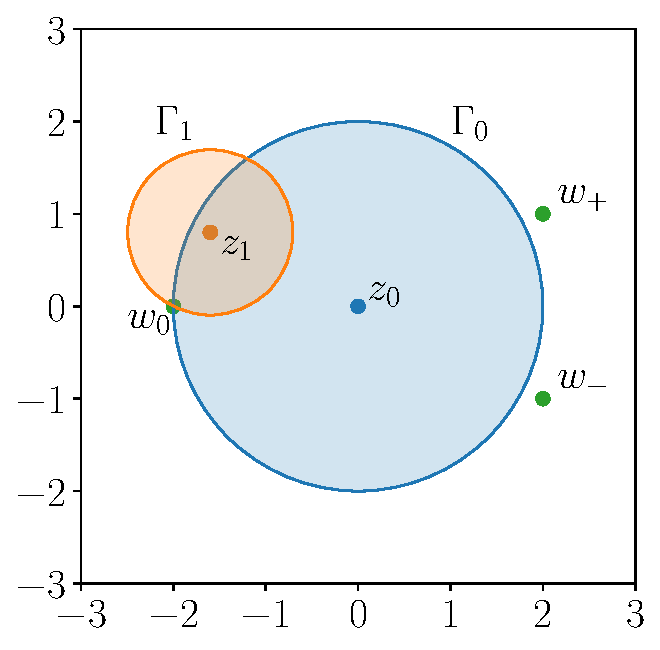
\includegraphics[width=0.5 \textwidth]{Images/analytic_continuation.pdf}
\caption{\label{fig:analcont}
  Example of analytic continuation.}
\end{figure}

In the case of simple poles in the homogeneous coefficient, we obtain a logarithmic behaviour of the solution, that requires some additional care in the analytic continuation.
The presence of logarithmic functions makes the solution multi-valued: it can be made single-valued by adding cuts in the complex plane, thus specifying the Riemann sheet where the function is evaluated.
This feature is clearly not present in the power series representation, but must be introduced to allow for a physical interpretation of the results.
To take it into account, we need to define in an unambiguous way the cut associated to each singularity that shows a logarithmic behaviour: their presence will then affect the process of analytic expansion.

In our example, we now consider a logarithmic behaviour in the points $w_0$, $w_\pm$, and we choose as the branch-cuts the horizontal lines parallel to the real axis that go from the singular point to $-\infty$.
In the following discussion we will always assume this convention,
which represents the standard choice for logarithmic branch cuts\footnote{This conventions is used, for instance, in {\sc Mathematica} by the function $\tt{Log[z]}$, for complex values of the variable $\tt{z}$.}.

\begin{figure}[t]
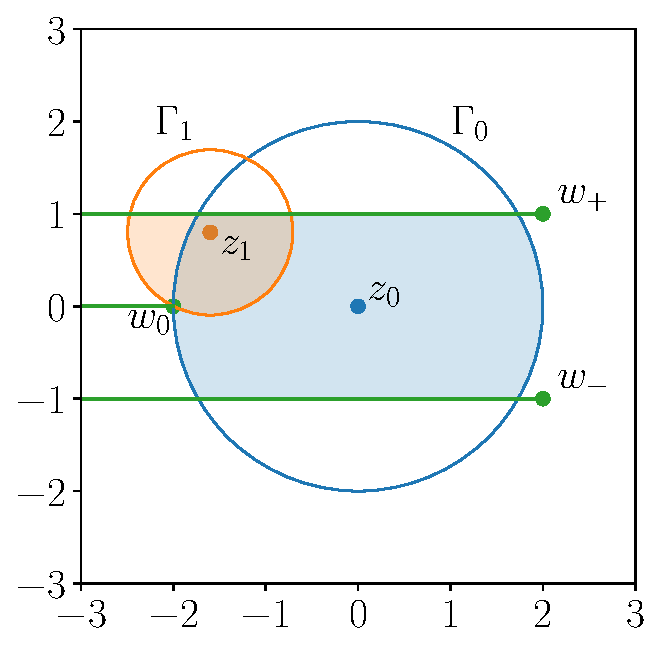
\includegraphics[width=0.49\textwidth]{Images/cuts_and_convergence.pdf}
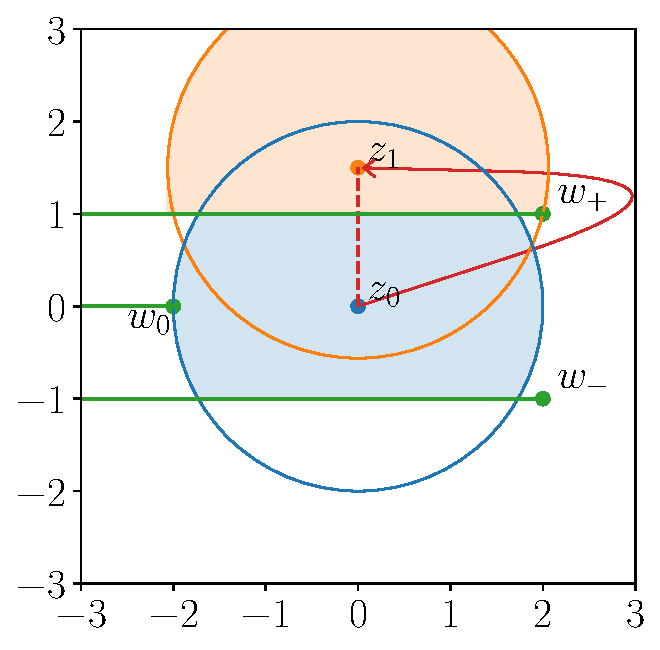
\includegraphics[width=0.49\textwidth]{Images/cuts_and_paths.pdf}
\caption{\label{fig:cuts}
 Example of the effect of branch-cuts on the convergence of the expanded solution: reduced convergence area (left) and different path for the analytic continuation (right).}
\end{figure}

The first consequence of the presence of branch-cuts in the procedure of analytic continuation is on the area of convergence of the series expansion.
While the proximity with a branch-cut does not modify the convergence radius of the series itself, it limits the area of the disc where the expansion converges to the desired value: 
once the cut is crossed, the series is evaluated on a Riemann sheet different than the one that we have chosen with the cuts, and thus the result can not be considered as the solution of the problem in the assigned domain.
This effect is illustrated on the left panel of Figure~\ref{fig:cuts}, that shows how the convergence discs $\Gamma_0$, $\Gamma_1$ introduced in Figure~\ref{fig:analcont} are modified once the branch cuts are inserted: while the discs themselves do not shrink, only the reduced highlighted area provides the correct evaluation of the solution.

The second consequence is on the path that is necessary to follow in order to extend the solution to an arbitrary point in the complex plane. The path has to be chosen in such a way that it does not cross any branch cut. This is illustrated on the right panel of Figure~\ref{fig:cuts}, where the dotted path from $z=0$ to $z_1$ is now forbidden by the presence of the branch cut corresponding to the pole $w_+$. The cut needs to be avoided with a path that goes around to the right of the singularity, as shown by the solid line. For the sake of readability, we have not drawn all the discs along the path, representing the intermediate steps of the analytic continuation.

\subsection{Choice of the path}
\label{subsec:path}
In the {\sc Mathematica} package {\sc SeaSyde}, we use the same convention for the branch-cuts as the one we introduced in the previous section, with branch-cuts parallel to the real axis and going from the singularities to $-\infty$.
As it has been shown in Section~\ref{sec:cuts}, with this choice the value of the solution in each point of the complex plane is unambiguously defined, as long as the path we use for the analytic continuation does not cross any branch-cut.
In the following, we briefly describe how such path can be defined when connecting two arbitrary points on the complex plane and the algorithm for its determination implemented within the package.
The analytic continuation described in the previous Section, moving in the complex plane of each kinematical invariant, allows to treat exactly in the same way the cases of real- and complex-valued masses. This represents the main remark of this paper.
\begin{figure}[t]
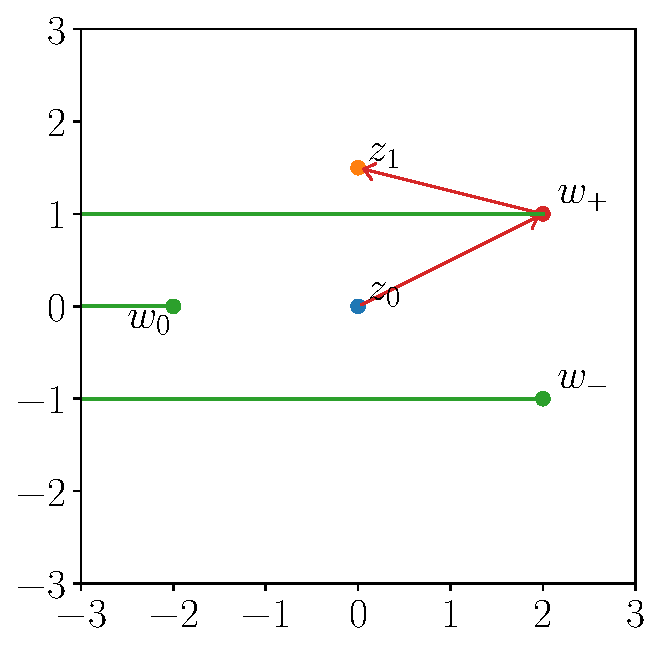
\includegraphics[width=0.49\textwidth]{Images/path_log.pdf}
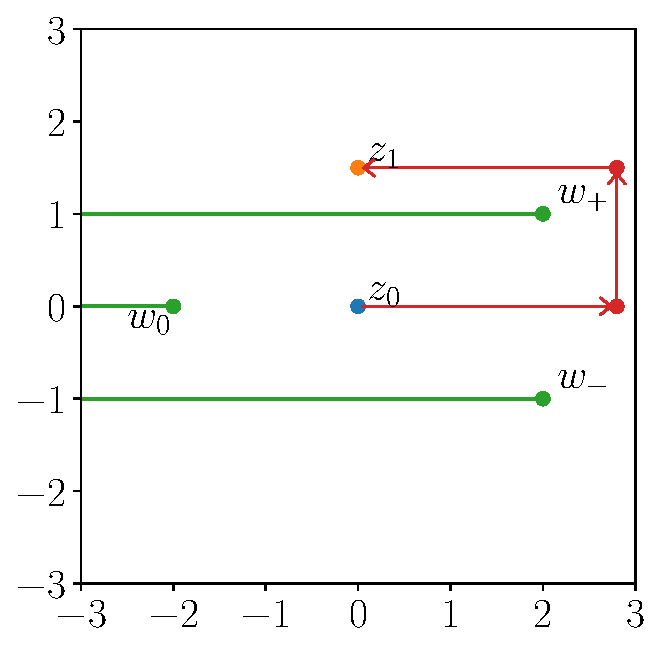
\includegraphics[width=0.49\textwidth]{Images/path_taylor.pdf}
\caption{\label{fig:path_logVStaylor}
 The two possible approaches in the definition of the path: the one requiring a logarithmic expansion (left) and the one only relying on the Taylor expansion (right).}
\end{figure}

There are two main approaches that can be used while defining the path: we can avoid the singularities or we can use them as an expansion point.
This two possibilities are illustrated in Figure~\ref{fig:path_logVStaylor}, where we consider once again the pole structure given by Eq.(\ref{eq:exampleeqdiff}), and we aim to move the boundary conditions from the point $z_0$ to the point $z_1$.
By choosing the singularity in $w_+$ as one of the possible expansion points, as shown in the left panel of Figure~\ref{fig:path_logVStaylor}, we obtain a logarithmic expansion around $w_+$, while if we avoid the singularity, as shown in the right panel of Figure~\ref{fig:path_logVStaylor}, we only rely on the ordinary Taylor expansion.
While leading exactly to the same result, the two approaches have different advantages and disadvantages.
By using the logarithmic expansion, we can expect a larger radius of convergence of the series, since the latter is not affected anymore by the presence of the pole upon which we are expanding: this can effectively reduce the number of steps required to reach the point of interest.
Furthermore, the presence of the branch-cut, starting from the singularity we are expanding upon, is automatically taken into account by the explicit logarithms appearing in the series.
On the other hand, in the current implementation of {\sc SeaSyde}, the expansion on a singular point requires a longer evaluation time with respect to the ordinary Taylor expansion on a regular point of the complex plane.
An optimised choice between the two different approaches thus requires to carefully balance these two effects.
In the physical applications we have dealt with while testing the code, we have observed how the presence of multiple singularities close to each other does not allow for a significant improvement of the convergence radius while using the logarithmic expansion. This fact has led us to prefer, for our final implementation, the more regular behaviour of the ordinary Taylor expansion.

With this choice, the algorithm to determine the path is straightforwardly implemented.
Since all the branch-cuts are parallel to each other and in the same direction, it is always possible to connect two arbitrary points on the complex plane with a path that goes around to the right of the rightmost singularity that lays between them, as it is shown in the right panel of Figure~\ref{fig:path_logVStaylor}. 

There is only one edge case that we need to discuss in more detail, that is the one in which the starting and ending point lay down on the same branch-cut, which is usually the real axis. In this case, indeed, there is an ambiguity, since it is not clear where the points are located with respect to the cut. This ambiguity can be discussed and solved in the light of the Feynman prescription for the particle propagators, which enforces the causality requirement of the theory.
If we consider, for the sake of simplicity, the propagator $\Pi(s)=i/(s-m^2+i\delta)$ of a massive scalar field, despite the kinematic invariant $s$ and the mass $m$ being real, the Feynman prescription shifts the first one to $s+i\delta$, i.e. in the upper half of the complex-$s$ plane.
Having a prescription which pushes the solution of the differential equation in one specific half of the complex-$z$ plane, removes any ambiguity associated with the evaluation of the function on the branching cut and allows us to uniquely determine the solution for any given BCs.
From a practical point of view, we might encounter two different scenarios: without or with poles between the start and the end points. In the first one the choice of the path is trivial and we can move directly from one point to the other, because, by construction, we are never crossing the cut. We can see this in the left panel of Figure~\ref{fig:realAxis}. 
\begin{figure}[t]
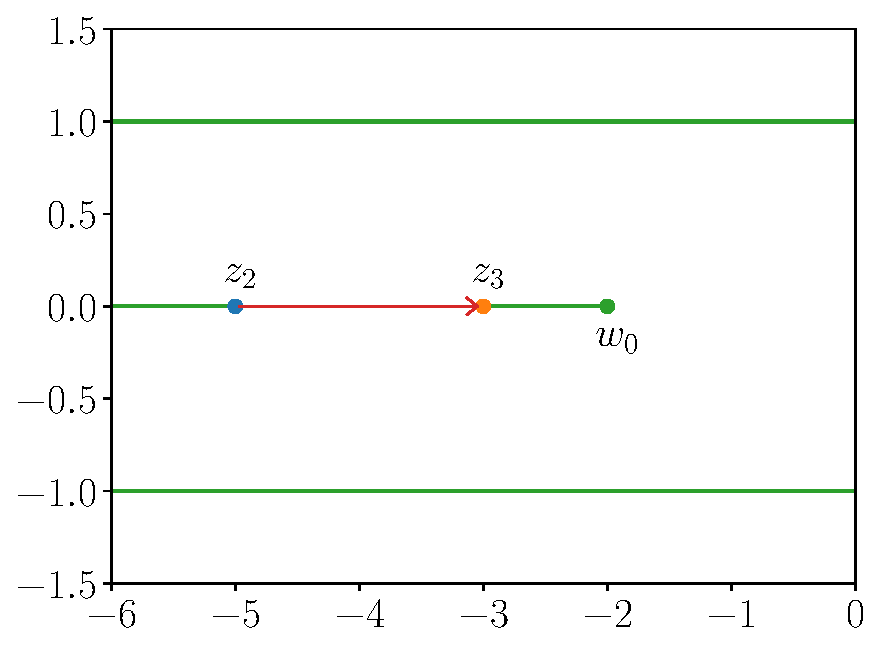
\includegraphics[width=0.49\textwidth]{paperSeaFire/Images/path_realaxis.pdf}
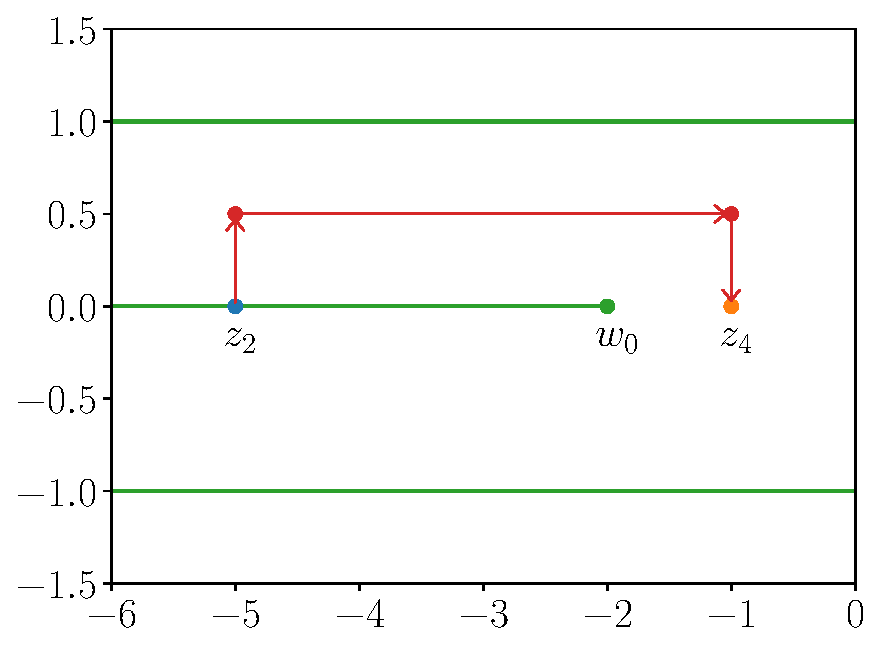
\includegraphics[width=0.49\textwidth]{paperSeaFire/Images/path_realaxis2.pdf}
\caption{\label{fig:realAxis}
Examples of two possible paths for linking two points laying on the same branch-cut: no singularities between them are present (left) or at least one is (right).}
\end{figure}
In the second one, instead, we could again either expand on the singularity or avoid it, as previously discussed. The choice we have made to avoid the singularities, however, forces us to adopt an horseshoe path, as depicted in the right panel of Figure~\ref{fig:realAxis}.
A prescription of $-i\delta$, on the contrary, would have implied an horseshoe in the lower half of the complex plane.
% While studying Feynman integrals with real internal masses, the poles are usually located on the real axis, that thus becomes a branch-cut starting from its rightmost singularity.
% Also the BCs and other points of interest usually assume real values, thus lying on the same branch-cut.
% The same situation might happen while considering the complex mass case: even if the poles are, in general, shifted on the complex plane, the boundary conditions and the point of interest might still accidentally lie on the same branch cut.
% If there is no pole between them, the path can simply connect them with a straight line: this approach does not lead to any ambiguity since the branch-cut is not problematic by itself, but it only leads to inconsistent results when it is crossed.
% On the other hand, an ambiguous situation is the one in which there is an additional pole located between them: if the path, in order to avoid the singularity, goes above or below the branch-cut, we obtain indeed two different results.
%We adopt the same prescription for the kinematic variables of the differential equation, which implies that the complete evolution of the solution from the BCs to the point of interest is performed not on the real axis, but in the complex plane of the kinematic variable, and, more precisely, in one specific half of that complex plane.
%{\color{red}
The prescription is not hard-coded within {\sc SeaSyde} and must be passed as an input parameter. As a consequence, the package can automatically perform the analytic continuation of the solution even if the user adopts different conventions.
%}
%We observe that the remark that we study the solution in the whole complex plane sets in a natural way the framework to handle Feynman integrals with internal complex masses.

\subsection{Solving a system of differential equations}
\label{sec:system}
%{\color{red}
The evaluation of a scattering amplitude requires the numerical calculation of a large set of Feynman integrals. Their number can range from a few, for one-loop corrections, to hundreds or thousands, for multi-loop ones. Fortunately not all of them are independent from each other.  Integration-by-Parts Identities \cite{Tkachov:1981wb,Chetyrkin:1981qh,Laporta:2001dd} allow us to express these integrals as a linear combination of MIs\footnote{Several computer implementations of the procedure are available \cite{Anastasiou:2004vj,Studerus:2009ye,vonManteuffel:2012np,Lee:2012cn,Lee:2013mka,Smirnov:2008iw,Smirnov:2014hma,Maierhoefer:2017hyi,Klappert:2020nbg}.}.

The computation of the MIs can be faced in different ways. One of these possibilities is by writing the system of first order linear differential equations with respect to the kinematical invariants $\mathbf{s}$, satisfied by the MIs. If $\vec{I}(\varepsilon,\mathbf{s})$ is a vector with the MIs of the problem under consideration as components, the systems can be expressed as follows:
\be
\label{eq:system}
\frac{\partial}{\partial s_\alpha} \vec{I}(\varepsilon,\mathbf{s})
= \mathbf{A}_\alpha(\varepsilon,\mathbf{s})\, \vec{I}(\varepsilon,\mathbf{s})\, ,
\ee
where $s_\alpha$ is one of the invariants, 
and $\mathbf{A}_\alpha(\varepsilon,\mathbf{s})$ is the matrix of the coefficients of the system, containing rational functions of all the invariants and depending upon the parameter $\varepsilon$. We look for a solution in form of a Laurent series in $\varepsilon$, $\vec{I}=\sum_{k=-N}^{\infty} \varepsilon^k \, \vec{I}^{(k)}$, where $N$ is the order of the maximal pole of the MIs. We substitute this form of the solution in Eq.~(\ref{eq:system}) and, order-by-order in $\varepsilon$, we study the resulting system of equations, starting from the one associated to the lowest power of the expansion in $\varepsilon$.

A particularly suitable situation is the one in which the choice of a basis of MIs yields systems of equations that, order-by-order in $\varepsilon$, are in triangular form. This allows for a straightforward solution of the problem. The solution of the system can proceed in cascade: we solve a first-order linear differential equation at a time, starting from the one that involves a single MI. The solution of this equation is plugged in the following one, that becomes a first-order non-homogeneous differential equation. Also the solution of the second equation is plugged, together with the solution of the first one, into the third equation, that in turn becomes a first-order non-homogeneous differential equation as well. We proceed in this way up to the complete solution of the system\footnote{This is the class of problems that can admit solutions in closed form, in terms of polylogarithmic functions.}.  
%In this case the different systems of equations are guaranteed to be, order by order in $\varepsilon$ in triangular form.}, but it is not necessary.
Each first-order differential equation can be solved using the procedure outlined in section~\ref{sec:example}, i.e. in a semi-analytic way.

%In this case the system can be solved using the procedure outlined in section~\ref{sec:example}. 
%The fact that now we have to deal with a system instead of a single differential equation increases the complexity of the system for the coefficients, equivalent to the one in Eq.(\ref{eq:example_syst}), which will now contain the coefficients of the series expansion of all the unknown master integrals. 

%The procedure outlined in section~\ref{sec:example} to solve a single differential equation can be generalised in a straightforward way to a system of differential equations as the one in Eq.(\ref{eq:system}).
%Such an extension comes at the price of an increased complexity of the system for the coefficients, equivalent to the one in Eq.(\ref{eq:example_syst}), which will now contain the coefficients of the series expansion of all the unknown master integrals. 

The {\sc Mathematica} package {\sc SeaSyde}, in its current implementation, can only solve systems of differential equations of this kind, i.e. in triangular form order-by-order in $\varepsilon$\footnote{
%The system simplifies further, if it is possible, by an appropriate change of basis, to cast it in the following differential form \cite{Henn:2013pwa}
%\be
%d\vec{J}=\varepsilon\, d\mathbf{\tilde A}\,\vec{J},\quad\quad
%\mathbf{\tilde A}=\sum_l \mathbf{\tilde A}_l \log l \, ,
%\label{can}
%\ee
%where $l$ are the letters, i.e. the combination of kinematic variables which parametrise the singular structure of the scattering amplitude and in particular the various internal thresholds and pseudo-thresholds of the Feynman integral. 
%The structure of equation \ref{can} is called $\varepsilon$-form or canonical form.
%A further important simplification of the problem is achieved if the choice of the MIs allows to cast the system of equations in canonical form \cite{Henn:2013pwa}. In this case the system becomes
%Now the $\varepsilon$ dependence of the matrices $\mathbf{A}$ comes out to be completely factorised. In this case it is customary to look for solutions in power series of $\varepsilon$, $\vec{J}=\sum_{k=0}^{\infty} \varepsilon^k \, \vec{J}^{(k)}$, re-scaling appropriately by a suitable power of $\varepsilon$ the masters when moving from the basis $\vec{I}$ of Eq.~(\ref{eq:system}) to the basis $\vec{J}$ of (\ref{can}) \cite{Henn:2014qga}.
Although the canonical form \cite{Henn:2014qga} of the system speeds up its semi-analytical solution, it is not mandatory for the use of {\sc SeaSyde}. It is indeed sufficient that the system admits different subsequent orders in $\varepsilon$ and at each of these orders the systems are in triangular form.
%(MIs decoupled in $\varepsilon$).
}. The algebraic procedure to write the system as a triangular matrix needs to be performed by the user.




In general, the systems of differential equations for a fixed order in $\varepsilon$ depend on multiple kinematic variables. We solve the problem by analysing only one of them at a time. 
In doing so, the dependence on all the other variables is parametric, and we reduce the problem to a system of differential equations in one variable.
The strategy adopted in  the package {\sc SeaSyde} is the following. Suppose that we are dealing with a problem depending upon two dimensionless variables, $x$ and $y$ . We ask {\sc SeaSyde} to evolve the solution from the point in which we fixed the boundary conditions, say $(x_0,y_0)$, to the point $(x_1,y_1)$. The solution of the problem will proceed solving the system in $x$, with a fixed value of $y=y_0$, from $x_0$ to $x_1$ and then solving the system in $y$ with $x=x_1$ from $y=y_0$ to $y=y_1$.
Integrating in $x$, at fixed $y=y_0$, the eventual cuts will depend on $y_0$. However, this value is fixed and then the cuts in the complex $x$ plane are given. To overcome the cuts, {\sc SeaSyde} uses the procedure outlined in section~\ref{sec:example}.
The same situation holds when we integrate in $y$ at fixed $x=x_1$. Now the eventual cuts will be in the complex $y$ plane and they will depend upon $x_1$, which is a fixed value. This means that also the cuts in $y$ are now given and {\sc SeaSyde} is able to overcome them with a path that moves at the right of the right-most branching point in $y$ (section~\ref{sec:example}).


%%%%%%%%%%%%%%% fine del blu








We can start to solve the system from the lowest order in the $\varepsilon$ expansion and work our way up to the desired order.



\begin{comment}


{\color{red}
For each MI, we can write the linear first-order differential equation with respect to one of the invariants which the integral depends upon.
 In the in-homogeneous term, we find additional integrals with simpler topologies, that can be written in terms of MIs by using the same reduction procedure previously introduced.
The problem is thus reduced to the solution of the complete system of differential equations satisfied by the integral of interest and all the relevant subtopologies, collectively represented by $\vec{I}(\mathbf{s})$, where  $\mathbf{s}$ represents all the kinematic variables. 

We have
\be
%\label{eq:system}
\frac{\partial}{\partial s_\alpha} \vec{I}(\varepsilon,\mathbf{s})
= \mathbf{A}_\alpha(\varepsilon,\mathbf{s})\, \vec{I}(\varepsilon,\mathbf{s})\, ,
\ee
where $s_\alpha$ is a generic kinematic variable and the coefficient matrix $\mathbf{A}_\alpha$ contains rational functions of all the invariants.

% {\color{red}
% In order to solve the system presented in Eq.(\ref{eq:system}) we can expand both $\vec{I}(\varepsilon,\mathbf{s})$ and $\mathbf{A}(\varepsilon,\mathbf{s})$ in $\varepsilon$, i.e.
% \be
% \vec{I}(\varepsilon,\mathbf{s})=\sum_{k=0}^{+\infty} \vec{I}^{(k)}(\mathbf{s})\varepsilon^k\;,\qquad
% \mathbf{A}(\varepsilon,\mathbf{s})=\sum_{k=0}^{+\infty} \mathbf{A}^{(k)}(\mathbf{s})\varepsilon^k.
% \label{eq:expansion}
% \ee
% Note that it is always possible to start the expansions from $k=0$ thanks either to a re-scaling $\vec{I}\to\varepsilon^m\vec{I}$ or an overall multiplication of the system for $\varepsilon^m$, with $m$ an appropriate integer. Substituting Eq.(\ref{eq:expansion}) in Eq.(\ref{eq:system}) and collecting order-by-order in $\varepsilon$ we obtain
% \be
% \frac{\partial}{\partial s_\alpha} \vec{I}^{(k)}(\mathbf{s}) = 
% \mathbf{A}^{(0)}(\mathbf{s})\vec{I}^{(k)}(\mathbf{s}) + 
% \sum_{j=0}^{k-1}\mathbf{A}^{(k-j)}(\mathbf{s})\vec{I}^{(j)}(\mathbf{s}).
% \label{eq:systemexpanded}
% \ee
% We can clearly see that in Eq.(\ref{eq:systemexpanded}), only $\vec{I}^{(j)}$, with $j<k$ appear. This means that we can start from the system for $k=0$, solve it and obtain $\vec{I}^{(0)}$. Now we substitute $\vec{I}^{(0)}$ into the equation for $\vec{I}^{(1)}$ and solve it with respect to $\vec{I}^{(1)}$. Then we can proceed recursively.
% }
The procedure outlined in section~\ref{sec:example} to solve a single differential equation can be generalised in a straightforward way to a system of differential equations as the one in Eq.(\ref{eq:system}).
Such an extension comes at the price of an increased complexity of the system for the coefficients, equivalent to the one in Eq.(\ref{eq:example_syst}), which will now contain the coefficients of the series expansion of all the unknown master integrals. 


%{\color{red} 
In general, the system of differential equations for a fixed order in $\varepsilon$ depends on multiple kinematic variables. However, we can considerably simplify the problem by analysing only one of them at a time. In doing so the dependency from all the other variables becomes a parametric one, and we reduce the problem to a system of differential equations in one variable.

The {\sc Mathematica} package {\sc SeaSyde}, in its current implementation, can only solve systems of differential equations provided, order-by-order in $\varepsilon$, in triangular form:
%canonical form.
%Furthermore, at the moment it only accepts as an input a system provided in triangular form: 
the algebraic procedure to write the system as a triangular matrix needs to be performed by the user.
We can start to solve the system from the lowest order in the $\varepsilon$ expansion and work our way up to the desired order.
}
%}
% In general, the system of differential equations obtained in this way depends on multiple kinematic variables, while we considered so far only one-dimensional differential equations.
% As a consequence, also the branch-cuts described in Section~\ref{sec:cuts} actually become surfaces in a higher-dimensional space and, in order to describe the path for the transport of the boundary conditions, the expansion with respect to more variables can be in principle needed.
% In our implementation we circumvent these complications by considering the evolution of a single variable at a time.
% With this approach, during each single expansion we are dealing with a one-dimensional problem, and all the remarks made in the previous sections still hold.

{\color{red}
An additional complication is given by the fact that, in practical applications, the computation is performed in dimensional regularisation, evaluating the integrals in $d=4-2\varepsilon$ dimensions.
This introduces in the equations and in the solutions an additional dependence on the regularisation parameter $\varepsilon$ which is in general non trivial and usually requires a Laurent expansion in $\varepsilon$ of the result in order to isolate its singular behaviour.

The system simplifies further, if it is possible, by an appropriate change of basis, to cast it in the following differential form \cite{Henn:2013pwa}
\be
d\vec{I}=\varepsilon\, d\mathbf{\tilde A}\,\vec{I},\quad\quad
\mathbf{\tilde A}=\sum_l \mathbf{\tilde A}_l \log l \, ,
\label{can}
\ee
%$\vec{I}\to \mathbf{B}\vec{I}$, to bring the coefficient matrix into the form $\mathbf{A}(\varepsilon,\mathbf{s})\to\varepsilon \mathbf{\tilde A}(\mathbf{s})$, 
called the $\varepsilon$-form or canonical form. In Eq.~(\ref{can}), the $\varepsilon$ dependence of the matrix of the system is completely factorised. $\mathbf{\tilde A}_l$ is a matrix of rational numbers and $l$ are the letters, i.e. the combination of kinematic variables which parameterise the singular structure of the scattering amplitude and in particular the various internal thresholds and pseudo-thresholds of the Feynman integral. The canonical basis $\vec{I}$ is expressed in Taylor series of $\varepsilon$, $\vec{I}=\sum_{k=0}^{\infty} \varepsilon^k \, \vec{I}^{(k)}$, 
and order by order in $\varepsilon$ the system (\ref{can}) is in triangular form. 
%We mean by ``decoupled'' a system that can be solved indeed solving a cascade of first-order differential equations,
%%The biggest advantage given by the canonical form is the fact that the system, order by order in $\varepsilon$, gets in upper-triangular form, 
%because the $n$-th equation contains only the MIs from the first $n-1$. 
In this case we can solve the system using a \textit{bottom-to-top} approach, that is we can solve the first equation, inside which appears only one unknown, then substitute the solution inside the second one and proceed recursively.
%In this case we the system can be written, in differential form, as
%\be
%d\vec{I}=\varepsilon\, d\mathbf{\tilde A}\,\vec{I},\quad\quad
%\mathbf{\tilde A}=\sum_l \mathbf{\tilde A}_l \log l
%\ee
%with $\mathbf{\tilde A}_l$ a matrix of rational numbers and $l$ the letters, i.e. the combination of kinematic variables which parametrise the singular structure of the scattering amplitude and in particular the various internal thresholds of the Feynman integral.
%The complete information about the singular structure of the problem under study, when it can be written in canonical form, is thus given by the set of the letters.
%The latter can be read from the matrix $\mathbf{\tilde A}$, in general after the application of a partial fractioning simplification procedure.
%
Writing the system in canonical form is particularly useful since it automatically decouples the equations of each order in $\varepsilon$. 

However, when the canonical basis is not available, we consider in any case that the system is in a form which is triangular at each order in $\varepsilon$.

%and with the differential equations that are not singular in the $\varepsilon \to 0$ limit.
%
The {\sc Mathematica} package {\sc SeaSyde}, in its current implementation, can only solve systems of differential equations provided, order-by-order in $\varepsilon$, in triangular form:
%canonical form.
%Furthermore, at the moment it only accepts as an input a system provided in triangular form: 
the algebraic procedure to write the system as a triangular matrix needs to be performed by the user.
We can start to solve the system from the lowest order in the $\varepsilon$ expansion and work our way up to the desired order.
}

\end{comment}